\documentclass[a4paper,11pt,fleqn,dvipsnames,twoside,openright]{memoir} 	% Openright aabner kapitler paa hoejresider (openany begge)

%%%% PACKAGES %%%%

% ¤¤ Oversaettelse og tegnsaetning ¤¤ %
\usepackage[utf8]{inputenc}					% Input-indkodning af tegnsaet (UTF8)
\usepackage[danish]{babel}					% Dokumentets sprog
\usepackage[T1]{fontenc}					% Output-indkodning af tegnsaet (T1)
\usepackage{ragged2e,anyfontsize}			% Justering af elementer
\usepackage{fixltx2e}						% Retter forskellige fejl i LaTeX-kernen
																			
% ¤¤ Figurer og tabeller (floats) ¤¤ %
\usepackage{graphicx} 						% Haandtering af eksterne billeder (JPG, PNG, EPS, PDF)
%\usepackage{eso-pic}						% Tilfoej billedekommandoer paa hver side
%\usepackage{wrapfig}						% Indsaettelse af figurer omsvoebt af tekst. \begin{wrapfigure}{Placering}{Stoerrelse}
\usepackage{multirow}                		% Fletning af raekker og kolonner (\multicolumn og \multirow)
\usepackage{multicol}         	        	% Muliggoer output i spalter
\usepackage{rotating}						% Rotation af tekst med \begin{sideways}...\end{sideways}
\usepackage{colortbl} 						% Farver i tabeller (fx \columncolor og \rowcolor)
\usepackage{xcolor}							% Definer farver med \definecolor. Se mere: http://en.wikibooks.org/wiki/LaTeX/Colors
\usepackage{flafter}						% Soerger for at floats ikke optraeder i teksten foer deres reference
\let\newfloat\relax 						% Justering mellem float-pakken og memoir
\usepackage{float}							% Muliggoer eksakt placering af floats, f.eks. \begin{figure}[H]

% ¤¤ Matematik mm. ¤¤
\usepackage{amsmath,amssymb,stmaryrd} 		% Avancerede matematik-udvidelser
\usepackage{mathtools,mathabx}
\newcommand\ARN[1]{\makebox[0pt][l]{$#1$}\kern-0.15em\raisebox{1.5ex}{$\curvearrowright$}}
\newcommand\ALN[1]{\makebox[0pt][l]{$#1$}\kern-0.15em\raisebox{1.5ex}{$\curvearrowleft$}}
\newcommand\AR[1]{\makebox[0pt][l]{$#1$}\kern0.0em\raisebox{1.5ex}{$\curvearrowright$}}
\newcommand\AL[1]{\makebox[0pt][l]{$#1$}\kern0.0em\raisebox{1.5ex}{$\curvearrowleft$}}						% Andre matematik- og tegnudvidelser
\usepackage{textcomp}                 		% Symbol-udvidelser (f.eks. promille-tegn med \textperthousand )
\usepackage{rsphrase}						% Kemi-pakke til RS-saetninger, f.eks. \rsphrase{R1}
\usepackage[version=3]{mhchem} 				% Kemi-pakke til flot og let notation af formler, f.eks. \ce{Fe2O3}
\usepackage{siunitx}						% Flot og konsistent praesentation af tal og enheder med \si{enhed} og \SI{tal}{enhed}
\sisetup{output-decimal-marker = {,}}		% Opsaetning af \SI (DE for komma som decimalseparator) 

% ¤¤ Referencer og kilder ¤¤ %
\usepackage[danish]{varioref}				% Muliggoer bl.a. krydshenvisninger med sidetal (\vref)
\usepackage{natbib}							% Udvidelse med naturvidenskabelige citationsmodeller
%\usepackage{xr}							% Referencer til eksternt dokument med \externaldocument{<NAVN>}
%\usepackage{glossaries}					% Terminologi- eller symbolliste (se mere i Daleifs Latex-bog)

% ¤¤ Misc. ¤¤ %
\usepackage{listings}						% Placer kildekode i dokumentet med \begin{lstlisting}...\end{lstlisting}
\usepackage{lipsum}							% Dummy text \lipsum[..]
\usepackage[shortlabels]{enumitem}			% Muliggoer enkelt konfiguration af lister
\usepackage{pdfpages}						% Goer det muligt at inkludere pdf-dokumenter med kommandoen \includepdf[pages={x-y}]{fil.pdf}	
\pdfoptionpdfminorversion=6					% Muliggoer inkludering af pdf dokumenter, af version 1.6 og hoejere
\pretolerance=2500 							% Justering af afstand mellem ord (hoejt tal, mindre orddeling og mere luft mellem ord)

% Kommentarer og rettelser med \fxnote. Med 'final' i stedet for 'draft' udloeser hver note en error i den faerdige rapport.
\usepackage[footnote,draft,danish,silent,nomargin]{fixme}		


%%%% CUSTOM SETTINGS %%%%

% ¤¤ Marginer ¤¤ %
\setlrmarginsandblock{3.5cm}{2.5cm}{*}		% \setlrmarginsandblock{Indbinding}{Kant}{Ratio}
\setulmarginsandblock{2.5cm}{3.0cm}{*}		% \setulmarginsandblock{Top}{Bund}{Ratio}
\checkandfixthelayout 						% Oversaetter vaerdier til brug for andre pakker

%	¤¤ Afsnitsformatering ¤¤ %
\setlength{\parindent}{0mm}           		% Stoerrelse af indryk
\setlength{\parskip}{3mm}          			% Afstand mellem afsnit ved brug af double Enter
\linespread{1,1}							% Linie afstand

% ¤¤ Litteraturlisten ¤¤ %
\bibpunct[,]{[}{]}{;}{a}{,}{,} 				% Definerer de 6 parametre ved Harvard henvisning (bl.a. parantestype og seperatortegn)
\bibliographystyle{bibtex/harvard}			% Udseende af litteraturlisten.

% ¤¤ Indholdsfortegnelse ¤¤ %
\setsecnumdepth{subparagraph}		 			% Dybden af nummerede overkrifter (part/chapter/section/subsection)
\maxsecnumdepth{subparagraph}					% Dokumentklassens graense for nummereringsdybde
\settocdepth{subparagraph} 					% Dybden af indholdsfortegnelsen

% ¤¤ Lister ¤¤ %
\setlist{
  topsep=0pt,								% Vertikal afstand mellem tekst og listen
  itemsep=-1ex,								% Vertikal afstand mellem items
} 

% ¤¤ Visuelle referencer ¤¤ %
\usepackage[colorlinks]{hyperref}			% Danner klikbare referencer (hyperlinks) i dokumentet.
\hypersetup{colorlinks = true,				% Opsaetning af farvede hyperlinks (interne links, citeringer og URL)
    linkcolor = black,
    citecolor = black,
    urlcolor = black
}

% ¤¤ Opsaetning af figur- og tabeltekst ¤¤ %
\captionnamefont{\small\bfseries\itshape}	% Opsaetning af tekstdelen ('Figur' eller 'Tabel')
\captiontitlefont{\small}					% Opsaetning af nummerering
\captiondelim{. }							% Seperator mellem nummerering og figurtekst
\hangcaption								% Venstrejusterer flere-liniers figurtekst under hinanden
\captionwidth{\linewidth}					% Bredden af figurteksten
\setlength{\belowcaptionskip}{0pt}			% Afstand under figurteksten
		
% ¤¤ Opsaetning af listings ¤¤ %

\definecolor{commentGreen}{RGB}{34,139,24}
\definecolor{stringPurple}{RGB}{208,76,239}

\lstset{language=Matlab,					% Sprog
	basicstyle=\ttfamily\scriptsize,		% Opsaetning af teksten
	keywords={for,if,while,else,elseif,		% Noegleord at fremhaeve
			  end,break,return,case,
			  switch,function},
	keywordstyle=\color{blue},				% Opsaetning af noegleord
	commentstyle=\color{commentGreen},		% Opsaetning af kommentarer
	stringstyle=\color{stringPurple},		% Opsaetning af strenge
	showstringspaces=false,					% Mellemrum i strenge enten vist eller blanke
	numbers=left, numberstyle=\tiny,		% Linjenumre
	extendedchars=true, 					% Tillader specielle karakterer
	columns=flexible,						% Kolonnejustering
	breaklines, breakatwhitespace=true,		% Bryd lange linjer
}

% ¤¤ Navngivning ¤¤ %
\addto\captionsdanish{
	\renewcommand\appendixname{Appendiks}
	\renewcommand\contentsname{Indholdsfortegnelse}	
	\renewcommand\appendixpagename{Appendiks}
	\renewcommand\appendixtocname{Appendiks}
	\renewcommand\cftchaptername{\chaptername~}				% Skriver "Kapitel" foran kapitlerne i indholdsfortegnelsen
	\renewcommand\cftappendixname{\appendixname~}			% Skriver "Appendiks" foran appendiks i indholdsfortegnelsen
}

% ¤¤ Kapiteludssende ¤¤ %
\definecolor{numbercolor}{gray}{0.7}		% Definerer en farve til brug til kapiteludseende
\newif\ifchapternonum

\makechapterstyle{jenor}{					% Definerer kapiteludseende frem til ...
  \renewcommand\beforechapskip{0pt}
  \renewcommand\printchaptername{}
  \renewcommand\printchapternum{}
  \renewcommand\printchapternonum{\chapternonumtrue}
  \renewcommand\chaptitlefont{\fontfamily{pbk}\fontseries{db}\fontshape{n}\fontsize{25}{35}\selectfont\raggedleft}
  \renewcommand\chapnumfont{\fontfamily{pbk}\fontseries{m}\fontshape{n}\fontsize{1in}{0in}\selectfont\color{numbercolor}}
  \renewcommand\printchaptertitle[1]{%
    \noindent
    \ifchapternonum
    \begin{tabularx}{\textwidth}{X}
    {\let\\\newline\chaptitlefont ##1\par} 
    \end{tabularx}
    \par\vskip-2.5mm\hrule
    \else
    \begin{tabularx}{\textwidth}{Xl}
    {\parbox[b]{\linewidth}{\chaptitlefont ##1}} & \raisebox{-15pt}{\chapnumfont \thechapter}
    \end{tabularx}
    \par\vskip2mm\hrule
    \fi
  }
}											% ... her

\chapterstyle{jenor}						% Valg af kapiteludseende - Google 'memoir chapter styles' for alternativer

% ¤¤ Sidehoved ¤¤ %

\makepagestyle{AAU}							% Definerer sidehoved og sidefod udseende frem til ...
\makepsmarks{AAU}{%
	\createmark{chapter}{left}{shownumber}{}{. \ }
	\createmark{section}{right}{shownumber}{}{. \ }
	\createplainmark{toc}{both}{\contentsname}
	\createplainmark{lof}{both}{\listfigurename}
	\createplainmark{lot}{both}{\listtablename}
	\createplainmark{bib}{both}{\bibname}
	\createplainmark{index}{both}{\indexname}
	\createplainmark{glossary}{both}{\glossaryname}
}
\nouppercaseheads											% Ingen Caps oenskes

\makeevenhead{AAU}{Gruppe B149}{}{\leftmark}				% Definerer lige siders sidehoved (\makeevenhead{Navn}{Venstre}{Center}{Hoejre})
\makeoddhead{AAU}{\rightmark}{}{Aalborg Universitet}		% Definerer ulige siders sidehoved (\makeoddhead{Navn}{Venstre}{Center}{Hoejre})
\makeevenfoot{AAU}{\thepage}{}{}							% Definerer lige siders sidefod (\makeevenfoot{Navn}{Venstre}{Center}{Hoejre})
\makeoddfoot{AAU}{}{}{\thepage}								% Definerer ulige siders sidefod (\makeoddfoot{Navn}{Venstre}{Center}{Hoejre})
\makeheadrule{AAU}{\textwidth}{0.5pt}						% Tilfoejer en streg under sidehovedets indhold
\makefootrule{AAU}{\textwidth}{0.5pt}{1mm}					% Tilfoejer en streg under sidefodens indhold

\copypagestyle{AAUchap}{AAU}								% Sidehoved for kapitelsider defineres som standardsider, men med blank sidehoved
\makeoddhead{AAUchap}{}{}{}
\makeevenhead{AAUchap}{}{}{}
\makeheadrule{AAUchap}{\textwidth}{0pt}
\aliaspagestyle{chapter}{AAUchap}							% Den ny style vaelges til at gaelde for chapters
															% ... her
															
\pagestyle{AAU}												% Valg af sidehoved og sidefod


%%%% CUSTOM COMMANDS %%%%

% ¤¤ Billede hack ¤¤ %
\newcommand{\figur}[4]{
		\begin{figure}[H] \centering
			\includegraphics[width=#1\textwidth]{billeder/#2}
			\caption{#3}\label{#4}
		\end{figure} 
}

% ¤¤ Specielle tegn ¤¤ %
\newcommand{\decC}{^{\circ}\text{C}}
\newcommand{\dec}{^{\circ}}
\newcommand{\m}{\cdot}


%%%% ORDDELING %%%%

\hyphenation{}											% Preamble indlaeses
\raggedbottom													% Soerger for at LaTeX ikke "straekker" teksten

%\includeonly{file1,file2}										% Inkluder kun specifikke filer (kommasepareret liste)

\begin{document}												% Starter dokumentet - obligatorisk


\frontmatter													% Forindhold - nummereres med romertal

\thispagestyle{empty}
\begin{flushright}
\vspace{3cm}

\phantom{hul}

\phantom{hul}

\phantom{hul}

\textsl{\Huge FUNDERING AF TILBYGNING AF STRØYBERGS PALÆ} \\ \vspace{1cm}

\rule{13cm}{3mm} \\ \vspace{1.5cm}
\vspace{1cm}

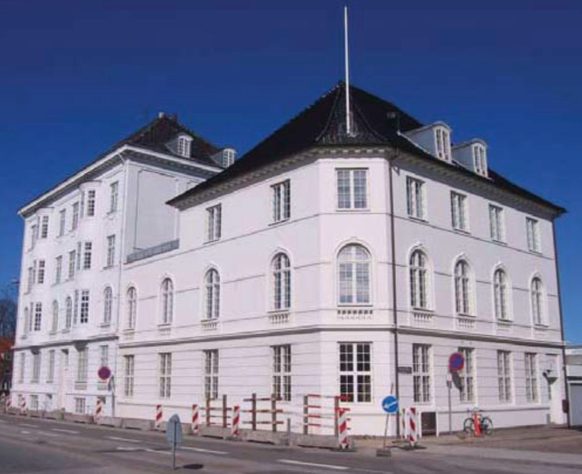
\includegraphics[width=0.9\textwidth]{billeder/forside.png}

\vspace{2cm} 
\textsc{\Large P2 Projekt - Modellernes virkelighed \\
Gruppe B149 \\
Byggeri \& Anlæg\\
Aalborg Universitet\\
D. 27. maj 2015\\}
\end{flushright}

\cleardoublepage												% Indsaetter tom side, saa naeste kapitel starter paa hoejre side (hvis noedvendigt)
% Dette er LaTeX-versionen af titelbladet for TNB studenterrapporter
% Filen kræver:
% Universitetets logo:  AAU-logo-stud-UK eller AAU-logo-stud-DK
% Synopsis: En fil ved navn synopsis.tex

% Udarbejdet af: Jesper Nørgaard (jesper@noergaard.eu) 10. april 2012

\phantomsection
\pdfbookmark[0]{Titelblad}{titelblad}
\thispagestyle{empty}

\begin{minipage}[t]{0.48\textwidth}
\vspace*{-25pt}			%\vspace*{-9pt}

\includegraphics[height=4cm]{billeder/AAU-logo-stud-DK-RGB}
\end{minipage}
\hfill
\begin{minipage}[t]{0.48\textwidth}
{\small 
\textbf{Første Studieår v/ Det Teknisk-}\\
\textbf{Naturvidenskabelige Fakultet}  \\
Byggeri og Anlæg \\
Strandvejen 12-14 \\
9000 Aalborg \\
http://www.tnb.aau.dk}
\end{minipage}

\vspace*{1cm}

\begin{minipage}[t]{0.48\textwidth}
\textbf{Titel:} \\[5pt]\bigskip\hspace{2ex}


\textbf{Projekt:} \\[5pt]\bigskip\hspace{2ex}
P2-projekt - Modellernes virkelighed

\textbf{Projektperiode:} \\[5pt]\bigskip\hspace{2ex}
Februar 2015 - Maj 2015

\textbf{Projektgruppe:} \\[5pt]\bigskip\hspace{2ex}
B149

\textbf{Deltagere:} \\[5pt]\hspace*{2ex}
Jacob Scharling Jørgensen \\\hspace*{2ex}
Karoline Vestergaard Hansen \\\hspace*{2ex}
Katrine Nørgaard Reberholt \\\hspace*{2ex}
Marc Lund Nielsen \\\hspace*{2ex}
Michael Elgaard Mortensen \\\hspace*{2ex}
Morten Rask Jensen \\\hspace*{2ex}
Nikolaj Skov Gravesen \\\bigskip\hspace{2ex}

\textbf{Vejledere:} \\[5pt]\hspace*{2ex}
Katrine Raabjerg Meltoft \\\hspace*{2ex}
Gitte \\\hspace*{2ex}
Johan \\\bigskip\hspace{2ex}

\vspace*{0.5cm}

\textbf{Oplagstal: 9} \\
\textbf{Sidetal: 79} \\
\textbf{Bilag: 4} \\ 
\textbf{Afsluttet 27-05-2015}

\end{minipage}
\hfill
\begin{minipage}[t]{0.483\textwidth}
Synopsis: \\[5pt]
\fbox{\parbox{7cm}{\bigskipDette P2-projekt omhandler den ene tilbygning til Strøybergs Palæ.
\newline
\newline
Strøybergs Palæ ligger placeret ved havnen i Aalborg og er placeret inden for en fremlagt vækstakse. Bygningen skal laves henfør lokalplan 1-1-107. Projektet beskriver tilbygningen ud fra to perspektiver; en kontekstuel del, hvor der lægges fokus på Aalborgs udvikling gennemtiden, og dens nuværende og planlagte udvikling, heriblandt den fremlagte vækstakse. Der vil blive redegjort for disse og diskuteret om den planlagte udvikling overhovedet er realistisk. Den tekniske del vil have fokus på dimensioneringen af tilbygningen og dens fundament. Der vil blive redegjort for Aalborgs geologi og forskellige jordarters udseende og styrke. Udfra dette vil der blive angivet en fundamenttype og udregnet størrelsen af det, så fundamentet har tilstrækkelig bæreevne til dimensioneringen af tilbygningen.
\bigskip}}
\end{minipage}

\vfill

{\footnotesize\itshape Rapportens indhold er frit tilgængeligt, men offentliggørelse (med kildeangivelse) må kun ske efter aftale med forfatterne.}

% Rapportens indhold er frit tilgængeligt, men offentliggørelse (med kildeangivelse) må kun ske efter aftale med forfatterne.
% The content of the report is freely available, but publication (with source reference) may only take place in agreement with the authors.

\cleardoublepage
\chapter*{Forord}
Denne rapport er udarbejdet af gruppe B149, en gruppe 2. semesters studerende på Byggeri og Anlæg uddannelsen ved Aalborg Universitet. \textit{Modellernes Virkelighed} er det overordnede tema for projektet, med undertemaet \textit{Vækstaksen i Aalborg}. Projektet omhandler en tilbygning ved Strøybergs Palæ.
\\
\\
Der rettes stor tak til vejledere Gitte Lyng Grønbech, Johan Clausen og Katrine Rabjerg Meltofte for vejledning og konstruktiv kritik. 
\\
\\
\textbf{Læsevejledning}
\newline
Der vil igennem rapporten fremtræde kildehenvisninger, og disse vil være samlet i en kildeliste bagest i rapporten. Der er i rapporten anvendt kildehenvisning efter Harvardmetoden. Denne henvisning fører til kildelisten, hvor bøger er angivet med forfatter, titel, udgave og forslag, mens internetsider er angivet med forfatter, titel og dato. Figurer og tabeller er nummereret i henhold til kapitel, dvs. den første figur i kapitel 7 har nummer 7.1, den anden nummer 7.2, osv. De samlede beregninger kan findes på hjemmesiden www.markhaurum.com, da der kun vil findes eksempler og korte uddrag af beregningerne i rapporten.


\phantom{Luft}

\phantom{Luft}

\begin{table}[H]
	\centering
		\begin{tabular}{c c c}
			\underline{\phantom{mmmmmmmmmmmmmm}} & \underline{\phantom{mmmmmmmmmmmmmm}} & \underline{\phantom{mmmmmmmmmmmmmm}} \\
			Jacob Scharling Jørgensen			& Karoline Vestergaard Hansen 		& Katrine Nørgaard Reberholt 			\\
			&&\\
			&&\\
			\underline{\phantom{mmmmmmmmmmmmmm}} & \underline{\phantom{mmmmmmmmmmmmmm}} & \underline{\phantom{mmmmmmmmmmmmmm}} \\
			Marc Lund Nielsen			& Michael Elgaard Mortensen 		& Morten Rask Jensen 				\\
			&&\\
			&&\\
		& \underline{\phantom{mmmmmmmmmmmmmm}} 	&			\\														
		& Nikolaj Skov Gravesen 							& 					
		\end{tabular}
\end{table}
\cleardoublepage

%%%% Indholdsfortegnelse (TOC) %%%%

\phantomsection													% Kunstigt afsnit, som hyperlinks kan 'holde fast i'
\pdfbookmark[0]{Indholdsfortegnelse}{indhold}					% Tildeler en klikbar bookmark til den endelige PDF
\tableofcontents*												% Indholdsfortegnelsen (kaldet ToC) 

%\addtocontents{toc}{\protect\newpage}							% Fremtvinger sideskift i ToC hvis noedvendig (der hvor koden placeres)


\mainmatter														% Hovedindhold - nummereres fra side 1

%%%% Rapportindhold %%%% 										% Rapportindholdet boer IKKE indeholde broedtekst - KUN includede filer!

%% Indledende %%												% Opdel evt. i passende afsnit for overblikkets skyld

\chapter{Indledning}
Aalborg Kommune er med et indbyggertal på over 205.000 og et areal på cirka  1.140 $km^2$, landets tredjestørste kommune målt på indbyggertal og landets anden største kommune målt på areal \citep{indbyggertal}. Det område, som Kommunen dækker, er vist på Figur \ref{fig:aalborgkommune}. 
\newline \indent{     }  Aalborg er en tidligere industriby og førhen var industriområderne placeret i Aalborg Centrum. Nye planer for Aalborg har ført denne industri ud i nogle yderpunkter af Aalborg by. Derfor har kommunen nye visioner om at flytte kultur, studieliv og turisme ind, hvor der før var industri. Kommunens visioner omkring byens udvikling fremgår af Kommuneplanen, hvor det primære fokus i denne rapport vil være et område gennem Aalborg, der er tiltænkt mest vækst, dette betegnes som Vækstaksen (se Figur \ref{fig:vaekstakse}).
\newline \indent{     }  Indenfor de seneste 5-10 år har Aalborgs centrale havnefront gennemgået en stor udvikling. Denne er stadig i gang, hvilket ses ved, at der kommer flere boligbyggerier til havnen, som Strøybergs Palæ er en del af. 
\newline \indent{     }  Det har siden år 2010 været på tale, at lave en tilbygning til den bevaringsværdige bygning, Strøybergs Palæ. Bygningen er fra år 1908 \citep{byggesagen}, beliggende centralt i Aalborg ved Slotspladsen, der er en cirka 200 meter vejstrækning og plads ved Aalborgs centrale havnefront, samt i nærheden af museet Utzon Centret og overfor shoppingcentret Friis. Figur \ref{fig:aalborg} viser Strøybergs Palæs beliggenhed. 
\newline \indent{     }  Når der skal anlægges nye arealer, bygninger, veje osv., skal det opføres i henhold til en lokalplan, der dækker et mindre område inden for kommunen, og har til formål at styre udviklingen indenfor dette område ved hjælp af fastlagte regler og målsætninger. Den gældende lokalplan for området ved Strøybergs Palæ er lokalplan 1-1-107. 

\begin{figure}[htbp] \centering
	\begin{minipage}[b]{0.48\textwidth}\centering
		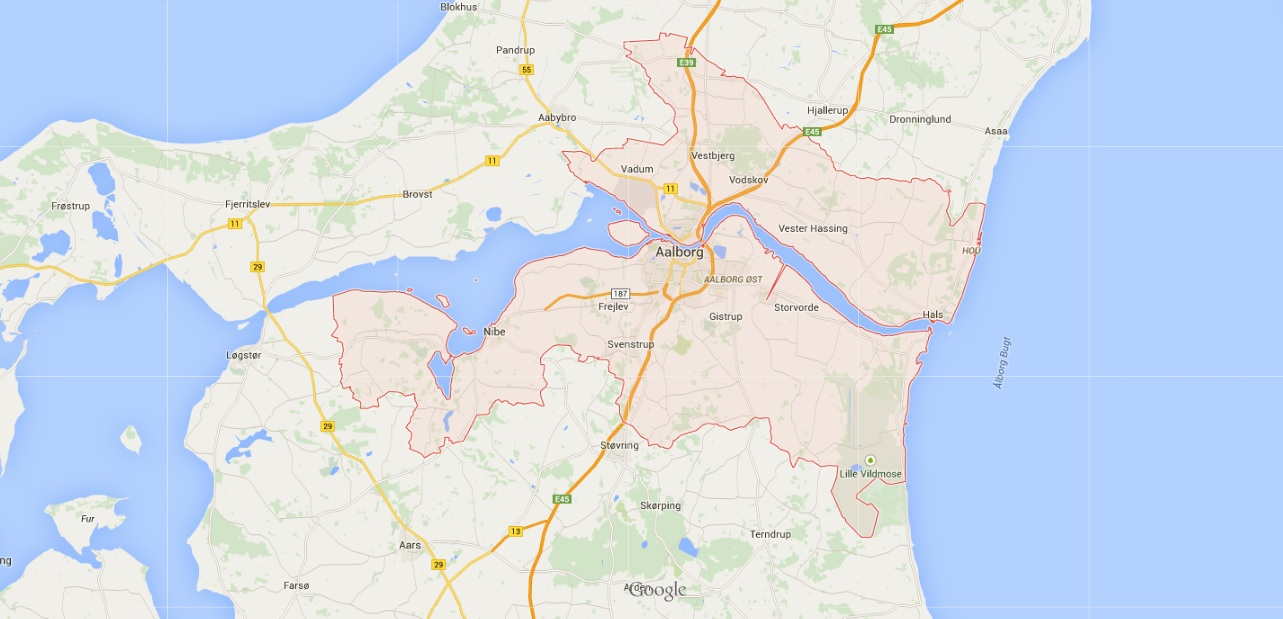
\includegraphics[width=1.0\textwidth]{billeder/aalborgkommune.png}
		\caption{Aalborg Kommune}
		\label{fig:aalborgkommune}
	\end{minipage}\hfill
	\begin{minipage}[b]{0.48\textwidth}\centering
		\centering
		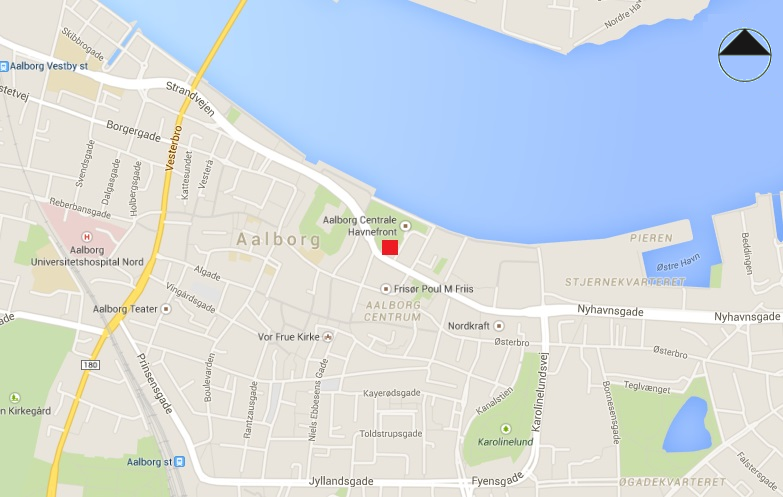
\includegraphics[width=1.0\textwidth]{billeder/aalborg.png}
		\caption{Strøybergs Palæs beliggenhed}
		\label{fig:aalborg}
	\end{minipage}
\end{figure}
\chapter{Problemformulering}

\section{Problemformulering og problemstillinger}
For at gennemføre planen om en tilbygning til Strøybergs Palæ kræves det, at lokalplanen for området stemmer overens med kommuneplanen. Ved konstruktionen af tilbygningen er det også nødvendigt at kende til geologien for området, for at bestemme hvilken type fundering, der skal benyttes. Dertil skal der anvendes en passende ståltype til dimensionering af stålprofilerne, for at tilbygningen har en tilstrækkelig bæreevne. Desuden skal der bestemmes en funderingstype til tilbygningen ud fra områdets geologi og jordbundsforhold. 

\begin{itemize} 
	\item Har Vækstaksen en betydning for tilbygningen af Strøybergs Palæ?
	\item Hvilken ståltype og stålprofil skal der anvendes ved tilbygningen til Strøybergs Palæ? 
	\item Hvilken funderingstype skal der benyttes ved området omkring Strøybergs Palæ? 
\end{itemize} 

\section{Problemafgrænsning}
Dette projekt beskriver tilbygningen af Strøybergs Palæ ud fra både et kontekstuelt og teknisk aspekt. I den kontekstuelle del lægges der vægt på beskrivelsen af Aalborg Kommuneplan samt udviklingen af områderne inden for Vækstaksen; hertil i særdeleshed området omkring havnefronten og Strøybergs Palæ, hvor Vækstaksens betydning for tilbygningen, samt tilbygningen relevans, diskuteres. Dertil beskrives og analyseres lokalplanen for området omkring Strøybergs Palæ, Lokalplan 1-1-107.
\newline \indent{     }  Den tekniske del belyser tilbygningen af Strøybergs Palæ ud fra to emner; konstruktionen af tilbygningen samt de geologiske forhold for området. I konstruktionsdelen opstilles der et statisk system for tilbygningen, som derefter dimensioneres for en række laster. 
\newline \indent{     }  Hertil beskrives de geologiske forhold, som gør sig gældende for Aalborg, hvortil der er foretaget jordbundsanalyser, for at finde frem til, hvilken type fundering der skal benyttes for tilbygningen.  

%% Kontekst %%



%% Teknisk %%



%% Afrunding %%

\chapter{Konklusion}
 Aalborg Kommune har igennem den nuværende kommuneplan en målsætning om, at blive Nordjyllands Vækstdynamo og være en by med fokus på udvikling af studieliv, erhverv, kultur m.m. Blandt et af kommunens fem fokuspunkter er “Aalborg - den attraktive storby”, som omhandler Vækstaksen, der beskriver et område i Aalborg, hvor der er stort fokus på byens udvikling og vækst.
 \newline \indent{     }  De seneste 10 års udvikling på Aalborg Havnefront har givet øget fokus på udviklingen i netop dette område. Strøybergs Palæs beliggenhed ved Aalborg Havnefront, i den mest centrale del af Vækstaksen, gør, at tilbygningen har gode vilkår i forbindelse med vækst og udvikling, og tilbygningen kan blandt andet bruges til beboelse og erhvervslokaler, som kan tiltrække nye virksomheder til området. Strøybergs Palæ er en lille del af Aalborgs udvikling, men en tilbygning må formodes ikke at have en central betydning for Aalborgs udvikling, idét tilbygningen kun er en lille del af Vækstaksen.
 \newline \indent{     }  Strøybergs Palæ er underlagt Lokalplan 1-1-107, der beskriver to byggefelter til bygningen. Der er udarbejdet en tilbygning for delområde B, hvor ny bebyggelse må opføres i 3 etager, samt en tagetage og kælder. Med udgangspunkt i Lokalplan 1-1-107 er bygningens størrelse og dimensioner bestemt. Hertil er der opstillet et statisk system, og der er valgt at indsætte tre stålrammer, hvor der dimensioneres efter den midterste ramme.
 \newline \indent{     }  Tilbygningens stålprofiler er dimensioneret ud fra ståltype S235 med profil nr. 450, samt ud fra de permanente og variable laster der virker på tilbygningen; egenlast, jordlast, vindlast, snelast og nyttelast. Herudfra er tilbygningens brud- og anvendelsesgrænsetilstand bestemt.
 \newline \indent{     }  Ud fra spændingstilstanden kan det konkluderes, at tilbygningen har en tilstrækkelig bæreevne, idet der fås en maksimal spænding på 100,51 MPa mod en flydespænding på 204,54 MPa. 
 \newline \indent{     }  For anvendelsesgrænsetilstanden er udbøjningen bestemt for tre af konstruktionens stålstænger. Her er den vandrette udbøjning bestemt til 1762,89 mm, mens den lodrette udbøjning er bestemt til 24,92 mm. Denne overskrider de anbefalede værdier for udbøjning af bærende konstruktioner, hvilke for vandret er 36 mm og lodret 15,63 mm.
 \newline \indent{     }  Tilbygningens fundament er dimensioneret ud fra Aalborgs geologi. Aalborgs undergrund er primært bestående af Aalborgler og funderingen til Strøybergs Palæ burde dermed være pælefundering. I dette projekt var ønsket at arbejde med direkte fundering, og derfor er der anvendt boreprofiler fra Hals, hvor undergrunden primært består af senglacialt sand, hvilket antages at være boreprofilerne fra området ved Strøybergs Palæ.
 \newline \indent{     }  De udførte laboratorieforsøg, hvor formålet er at bestemme friktionsvinklen, er udført på baskarpsand fra Sverige, der antages at være sandet fra boreprofilerne. Ud fra de fire forsøg er friktionsvinklen skønnet til $32,33^{\circ}$, der anvendes i videre beregninger af fundamentets størrelse. Der laves et punktfundament for hver søjle i det statiske system, med en længde og bredde på 0,94 m.


%%%% Kilder %%%%

\begingroup
	\raggedright
	\bibliography{bibtex/litteratur}							% Litteraturlisten inkluderes
\endgroup



%%%% Appendiks %%%%

\appendix														% Appendiks/bilag start - giver chapter bogstaver i stedet for tal
\clearforchapter												% Sikrer at pagestylen aktiveres paa den rigtige side
\phantomsection													% Kunstigt afsnit, som hyperlinks kan 'holde fast i'
\pdfbookmark[0]{Appendiks}{appendiks}							% Tildeler en klikbar bookmark til den endelige PDF

%% Indstillinger for appendiks (deaktiveret med "%") %%

%\pagestyle{empty}												% Sidehoved/-fod for standardsider aendres til tom for appendiks
%\aliaspagestyle{chapter}{empty}								% Sidehoved/-fod for kapitelsider aendres til tom for appendiks
%\settocdepth{chapter}											% Kun kapitel-niveau vises i ToC
%\addtocontents{toc}{\protect\cftpagenumbersoff{chapter}}		% Sidetal for kapitler fjernes i ToC

%% Filer til appendiks %%



%%%% Bilag %%%%

\chapter{Bilag}

%\phantomsection												% Kunstigt afsnit, som hyperlinks kan 'holde fast i'
%\addcontentsline{toc}{chapter}{Bilag A \ Navn} 				% Manuelle indgange i indholdsfortegnelsen (naar \includepdf bruges)

%\includepdf[pages={x-y}]{filnavn}								% Inkluder eksterne bilag med \includepdf[pages={x-y}]{filnavn}

\end{document}													% Slutter dokumentet - obligatorisk